\documentclass[11pt,a4paper,oneside]{article}
\usepackage{geometry}
\geometry{
	left=1.5cm, %% canh giữa hình
	right=1.5cm,
	top=2cm,
	bottom=2cm,
}
%ver-texlive2021
\usepackage{amsmath,amssymb,mathrsfs,fancyhdr,enumerate,multirow,makecell,currfile,venndiagram}
\usepackage{tikz-3dplot,tikz,tkz-tab,tabvar}
\usepackage{tabularx}
\usetikzlibrary{arrows,calc,intersections,angles,snakes,quotes,backgrounds,shapes.geometric,patterns}
\usepackage{pgfplots}
\pgfplotsset{compat=1.9}
\usepgfplotslibrary{fillbetween}
\usepackage[tikz]{bclogo}
\usepackage{ex_test}
\usepackage{times}

\setlength{\columnseprule}{1pt} 
	\usepackage{tabularx,array}
	\usepackage{fancyhdr}
	\pagestyle{fancy}
	\fancyhead{} 
	\fancyfoot{} 
	\fancyfoot[C]{\thepage/2 - Mã đề 9892} 
	\renewcommand{\headrulewidth}{0pt} 
\renewcommand{\nameex}{\color{black}Câu}
\begin{document}
	
%\begin{minipage}[t]{0.38\textwidth}
%	\begin{center}
%	{\large\bfseries SỞ GD\&ĐT TP. HỒ CHÍ MINH\\
%	TRƯỜNG THPT HỒ THỊ BI}\\[0.6em]
%\rule{3.6cm}{0.8pt}\\[-0.2em]
%{\itshape (Đề kiểm tra có 02 trang)}	
%	\end{center}
%\end{minipage}\hfill
%\begin{minipage}[t]{0.45\textwidth}
%	\centering
%	{\Large\bfseries ĐỀ KIỂM TRA GIỮA HỌC KỲ 1}\\[-0.15em]
%	{\Large\bfseries NĂM HỌC 2025 -- 2026}\\[-0.15em]
%	{\Large\bfseries MÔN TOÁN -- Khối lớp 11}\\[0.25em]
%	{\bfseries Thời gian làm bài : 60 phút}\\[-0.15em]
%	{(không kể thời gian phát đề)}
%\end{minipage}

\begin{minipage}[t]{0.38\textwidth}
	\begin{center}
		{\large\bfseries TUYỂN TẬP CÁC BÀI TOÁN HAY PHẦN HÀM SỐ\\
			Sưu tầm: Trương Nguyễn Phước Tâm}
	\end{center}
\end{minipage}\hfill

\vspace{0.8em}
	\renewcommand{\arraystretch}{1.2}
	\begin{tabularx}{\textwidth}{@{}>{\raggedright\arraybackslash}X@{}>{\raggedleft\arraybackslash}m{4.5cm}@{}}
	\textbf{Họ và tên học sinh :} \dotfill\quad
	\textbf{Số báo danh :} \dotfill
	&
	\centering
	\begin{tikzpicture}[baseline=(T.base)]
	\node[draw,rounded corners=2pt,thick,inner xsep=10pt,inner ysep=6pt] (T)
	{{\bfseries Mã đề} \textbf{00798}};
	\end{tikzpicture}
	\end{tabularx}
\vspace{0.1cm}
\noindent\rule{\textwidth}{1pt}
\textbf{PHẦN I. ( 4,0 điểm) Câu hỏi trắc nghiệm nhiều phương án lựa chọn.} Học sinh trả lời từ câu 1 đến câu 16. Mỗi câu hỏi học sinh chỉ chọn một phương án.

	\begin{multicols}{2}
	\begin{ex}
	Cho góc lượng giác $\alpha$ thỏa mãn $\sin \alpha = -\dfrac{4}{5}$ và $\pi < \alpha < \dfrac{3\pi}{2}$ Giá trị của $\cos \alpha$ bằng
	\choice
	{$-\dfrac{3}{5}$}
	{$-\dfrac{3}{25}$}
	{$\dfrac{9}{25}$}
	{$\dfrac{3}{5}$}
	\loigiai{
	% Nội dung lời giải
	}
	\end{ex}
	\begin{ex}
	Trên đường tròn bán kính $5 (\text{cm})$, xét một cung có độ dài bằng $10 (\text{cm})$ Số đo radian của góc ở tâm chắn cung tròn đó là
	\choice
	{$5 (\text{rad})$}
	{$2 (\text{rad})$}
	{$4 (\text{rad})$}
	{$3 (\text{rad})$}
	\loigiai{
	% Nội dung lời giải
	}
	\end{ex}
	\begin{ex}
	Cho $\sin a = \dfrac{2}{5}$ Khi đó $\cos 2a$ bằng
	\choice
	{$\dfrac{17}{25}$}
	{$\dfrac{17}{5}$}
	{$-\dfrac{3}{5}$}
	{$\dfrac{3}{5}$}
	\loigiai{
	% Nội dung lời giải
	}
	\end{ex}
	\begin{ex}
	Trong không gian cho hai đường thẳng $a, b$ cùng thuộc một mặt phẳng và không có điểm chung Khẳng định nào dưới đây đúng
	\choice
	{$a$ và $b$ trùng nhau}
	{$a$ và $b$ chéo nhau}
	{$a$ và $b$ song song}
	{$a$ và $b$ cắt nhau}
	\loigiai{
	% Nội dung lời giải
	}
	\end{ex}
	\begin{ex}
	Nghiệm của phương trình $\sin x = 1$ là
	\choice
	{$x = k\pi, k \in \mathbb{Z}$}
	{$x = k\pi, k \in \mathbb{Z}$} % Lưu ý: Đáp án A và B có nội dung giống nhau trong ảnh
	{$x = \dfrac{\pi}{2} + k\pi, k \in \mathbb{Z}$}
	{$x = \dfrac{\pi}{2} + k2\pi, k \in \mathbb{Z}$}
	\loigiai{
	% Nội dung lời giải
	}
	\end{ex}
	\begin{ex}
	Trong các khẳng định dưới đây, khẳng định nào sai
	\choice
	{$\sin(\pi - \alpha) = \sin \alpha$}
	{$\cos(\pi + \alpha) = \cos \alpha$}
	{$\sin(\pi + \alpha) = -\sin \alpha$}
	{$\cos(\pi - \alpha) = -\cos \alpha$}
	\loigiai{
	% Nội dung lời giải
	}
	\end{ex}
	\begin{ex}
	Trong các công thức lượng giác dưới đây, công thức nào đúng
	\choice
	{$\tan(a - b) = \dfrac{\tan a - \tan b}{1 + \tan a \tan b}$}
	{$\tan(a - b) = \dfrac{\tan a - \tan b}{1 - \tan a \tan b}$} % Lưu ý: Đáp án A và B khác nhau ở dấu +/-, nhưng cách trình bày trong ảnh có thể gây nhầm lẫn. Tôi lấy theo nội dung B
	{$\tan(a - b) = \dfrac{\tan a - \tan b}{\tan a - \tan b}$} % Nội dung này rất lạ, tôi cố gắng theo ảnh
	{$\tan(a - b) = \dfrac{\tan a - \tan b}{\tan a + \tan b}$} % Nội dung này rất lạ, tôi cố gắng theo ảnh
	\loigiai{
	% Nội dung lời giải
	}
	\end{ex}
	\begin{ex}
	Nghiệm của phương trình $\cos x = 0$ là
	\choice
	{$x = k\pi, k \in \mathbb{Z}$}
	{$x = k2\pi, k \in \mathbb{Z}$}
	{$x = \dfrac{\pi}{2} + k\pi, k \in \mathbb{Z}$}
	{$x = \dfrac{\pi}{2} + k2\pi, k \in \mathbb{Z}$}
	\loigiai{
	% Nội dung lời giải
	}
	\end{ex}
	\begin{ex}
	Tập xác định của hàm số $y = \cot x$ là
	\choice
	{$\mathbb{R} \setminus \left\{ \dfrac{\pi}{2} + k2\pi \Big| k \in \mathbb{Z} \right\}$}
	{$\mathbb{R} \setminus \left\{ \dfrac{\pi}{2} + k\pi \Big| k \in \mathbb{Z} \right\}$}
	{$\mathbb{R} \setminus \left\{ k\pi \Big| k \in \mathbb{Z} \right\}$}
	{$\mathbb{R} \setminus \left\{ k2\pi \Big| k \in \mathbb{Z} \right\}$}
	\loigiai{
	% Nội dung lời giải
	}
	\end{ex}
	\begin{ex}
	Một hình chóp với đáy là một ngũ giác có số mặt và số cạnh là
	\choice
	{$6$ mặt, $5$ cạnh}
	{$6$ mặt, $10$ cạnh}
	{$5$ mặt, $5$ cạnh}
	{$5$ mặt, $10$ cạnh}
	\loigiai{
	% Nội dung lời giải
	}
	\end{ex}
	\begin{ex}
	Góc có số đo $\dfrac{2\pi}{5} (\text{rad})$ đổi sang độ là
	\choice
	{$135^\circ$}
	{$240^\circ$}
	{$270^\circ$}
	{$72^\circ$}
	\loigiai{
	% Nội dung lời giải
	}
	\end{ex}
	\begin{ex}
	Cho tứ diện $ABCD$ Khẳng định nào dưới đây đúng
	\choice
	{$AB$ và $CD$ chéo nhau}
	{$AB$ và $CD$ song song với nhau}
	{Tồn tại một mặt phẳng chứa $AB$ và $CD$}
	{$AB$ và $CD$ cắt nhau}
	\loigiai{
	% Nội dung lời giải
	}
	\end{ex}
	\begin{ex}
	Trong không gian, khẳng định nào dưới đây đúng và đầy đủ nhất
	\choice
	{Qua $3$ điểm phân biệt bất kì, có duy nhất một mặt phẳng}
	{Qua $4$ điểm phân biệt bất kì, có duy nhất một mặt phẳng}
	{Qua $3$ điểm không thẳng hàng, có duy nhất một mặt phẳng}
	{Qua $2$ điểm phân biệt bất kì, có duy nhất một mặt phẳng}
	\loigiai{
	% Nội dung lời giải
	}
	\end{ex}
	\begin{ex}
	Trong các công thức lượng giác dưới đây, công thức nào sai?
	\choice
	{$\cos 2a = 2 \cos a$}
	{$\cos 2a = 2 \cos^2 a - 1$}
	{$\cos 2a = 1 - 2 \sin^2 a$}
	{$\cos 2a = \cos^2 a - \sin^2 a$}
	\loigiai{
	% Nội dung lời giải
	}
	\end{ex}
	\begin{ex}
	Cho góc lượng giác $\alpha$ thỏa mãn $\dfrac{3\pi}{2} < \alpha < 2\pi$. Khẳng định nào dưới đây đúng?
	\choice
	{$\sin \alpha > 0$}
	{$\tan \alpha > 0$}
	{$\cot \alpha > 0$}
	{$\cos \alpha > 0$}
	\loigiai{
	% Nội dung lời giải
	}
	\end{ex}
	\begin{ex}
		Đường cong trong hình sau đây là đồ thị của hàm số $y = \sin x$ trên đoạn $[-2\pi; 2\pi]$: 
			\vspace{-0.5cm}
			\begin{center}
			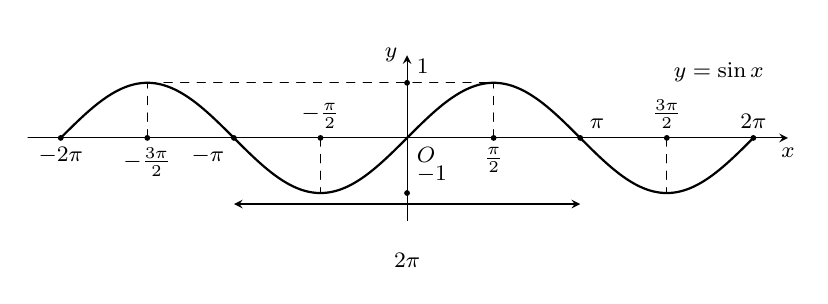
\begin{tikzpicture}[line join = round, line cap=round,>=stealth,font=\footnotesize,scale=0.7,samples=2000]
				\clip (-2*pi-0.6,-2.5) rectangle (2*pi+0.85,2);
				% Vẽ trục tọa độ
				\draw[->] (-2.2*pi, 0) -- (2.2*pi, 0) node[below] {$x$};
				\draw[->] (0, -1.5) -- (0, 1.5) node[left] {$y$};
				% Vẽ đồ thị hàm số y = sin(x)
				\draw[thick, smooth, domain=-2*pi:2*pi, variable=\x] plot ({\x}, {sin(\x r)});
				% Ghi nhãn phương trình
				\node at (1.8*pi, 1.2) {$y = \sin x$};
				% Các điểm và nhãn trên trục y và gốc tọa độ
				\node[below right] at (0,0) {$O$};
				\fill (0, 1) circle (1.5pt) node[above right] {$1$};
				\fill (0, -1) circle (1.5pt) node[above right] {$-1$};
				\fill (pi,0) circle (1.5pt) node[above right] {$\pi$};
				\fill (pi/2,0) circle (1.5pt) node[below] {$\frac{\pi}{2}$};
				\fill (3*pi/2,0) circle (1.5pt) node[above] {$\frac{3\pi}{2}$};
				\fill (2*pi,0) circle (1.5pt) node[above] {$2\pi$};
				\fill (-pi,0) circle (1.5pt) node[below left] {$-\pi$};
				\fill (-pi/2,0) circle (1.5pt) node[above] {$-\frac{\pi}{2}$};
				\fill (-3*pi/2,0) circle (1.5pt) node[below] {$-\frac{3\pi}{2}$};
				\fill (-2*pi,0) circle (1.5pt) node[below] {$-2\pi$};
				% Các đường nét đứt
				% Đường gióng dọc từ trục x tới các điểm cực trị
				\draw[dashed] (-1.5*pi, 0) -- (-1.5*pi, 1);
				\draw[dashed] (-0.5*pi, 0) -- (-0.5*pi, -1);
				\draw[dashed] (0.5*pi, 0) -- (0.5*pi, 1);
				\draw[dashed] (1.5*pi, 0) -- (1.5*pi, -1);
				\draw[dashed] (-1.5*pi, 1) -- (0.5*pi, 1);
				% Mũi tên chỉ chu kỳ 2π
				\draw[<->] (-pi, -1.2) -- (pi, -1.2) node[midway, below=0.5cm] {$2\pi$};
			\end{tikzpicture}
		\end{center}
	\vspace{-0.5cm}
		Khẳng định nào dưới đây sai?
	\choice	
	{Hàm số $y = \sin x$ là hàm số tuần hoàn với chu kì $T = 2\pi$}
	{Hàm số $y = \sin x$ đồng biến trên khoảng $\left(-\frac{\pi}{2}; \frac{\pi}{2}\right)$}
	{Hàm số $y = \sin x$ có tập giá trị là $[-1; 1]$}
	{Hàm số $y = \sin x$ là hàm số chẵn}
	
	\loigiai{
		
	}
	\end{ex}
	\end{multicols}	
\noindent \textbf{PHẦN II. (2,0 điểm) Câu hỏi trắc nghiệm đúng sai.} Học sinh trả lời từ câu 1 đến câu 2. Trong mỗi ý a), b), c), d) ở mỗi câu, học sinh chọn đúng hoặc sai.
\setcounter{ex}{0}
	\begin{ex}
Cho hình chóp $S.ABCD$ có đáy $ABCD$ là hình bình hành. Gọi $O$ là giao điểm của $AC$ và $BD$, $M$ là trung điểm của cạnh $SA$ (tham khảo hình vẽ):
\choiceTF[t]
{Đường thẳng $MC$ đi qua trung điểm của tam giác $SBD$}
{Đường thẳng $SO$ là giao tuyến của hai mặt phẳng $(SAC)$ và $(SBD)$}
{Nếu $(MBC) \parallel (SAD)$ thì $d$ đi qua trung điểm của cạnh $SD$}
{Hai đường thẳng $BC$ và $SD$ cắt nhau}
	\loigiai{
	% Nội dung lời giải
	}
	\end{ex}
	\begin{ex}
Cho góc lượng giác $\alpha$ thỏa mãn $\tan \alpha = 3$.
	\choiceTF[t]
	{$\cot \alpha = \dfrac{1}{3}$}
	{$\tan(\alpha + 3\pi) = 3 + 3\pi$}
	{$\tan(-\alpha) = -3$}
	{$\cot 2\alpha = -\dfrac{4}{3}$}
	\loigiai{
	% Nội dung lời giải
	}
	\end{ex}
\textbf{PHẦN III. (4,0 điểm) Tự luận.} Học sinh trả lời từ câu 1 đến câu 3.
\setcounter{ex}{0}
	\begin{ex}
 Giải phương trình lượng giác sau: $\cos \left( 2x - \dfrac{\pi}{3} \right) = \dfrac{\sqrt{3}}{2}$.
	\loigiai{
	% Nội dung lời giải
	}
	\end{ex}
	\begin{ex}
Hằng ngày mực nước của một con kênh lên xuống theo thủy triều. Chiều cao của mực nước trong kênh được mô hình hóa bởi hàm số $h(t) = 3 \cos \left( \dfrac{\pi t}{12} + \dfrac{\pi}{3} \right) + 10$, trong đó $h(t)$ là độ cao tính bằng centimet của mực nước trong kênh tính trung bình tại thời điểm $t$ (giờ) trong một ngày. Hỏi tại thời điểm nào trong ngày thì mực nước của con kênh đạt độ cao lớn nhất?
	\loigiai{
	% Nội dung lời giải
	}
	\end{ex}
	\begin{ex}
Cho hình chóp $S.ABCD$ có đáy là hình bình hành $ABCD$. Gọi $G$ là trung điểm của $AB$ và $G$ là trọng tâm của tam giác $SAB$. Lấy điểm $M$ trên cạnh $AD$, điểm $N$ trên cạnh $HC$ sao cho $AD = 3AM, HC = 3HN$.
	\begin{enumerate}[a)]
	\item Tìm giao tuyến của mặt phẳng $(SAC)$ và $(SBD)$.
	\item Gọi $P$ là giao điểm của $NG$ và mặt phẳng $(SAD)$. Chứng minh $G$ là trung điểm của $PN$.
	\end{enumerate}
	\loigiai{
	% Nội dung lời giải
	}
	\end{ex}

	\centerline{\textbf{----- HẾT -----}}
\end{document} 